\chapter{Discussion of Results}
\label{ch:discussion}

%TODO: Idee: Attention visualisieren am Anfang und am Ende des Transformers: Hat er während des Trainings gelernt?

\section{Hyper Parameter Optimization}

The following presents the results of the hyper parameter optimization on GermEval-2017 Task C and the Organic-2019 Coarse category dataset. We evaluate the performance of Hyperopt compared to a random search. Then, the next sections show how certain parameters impact the model performance. 

\subsection{Hyperopt Evaluation}

\begin{figure}[ht]
	\centering
	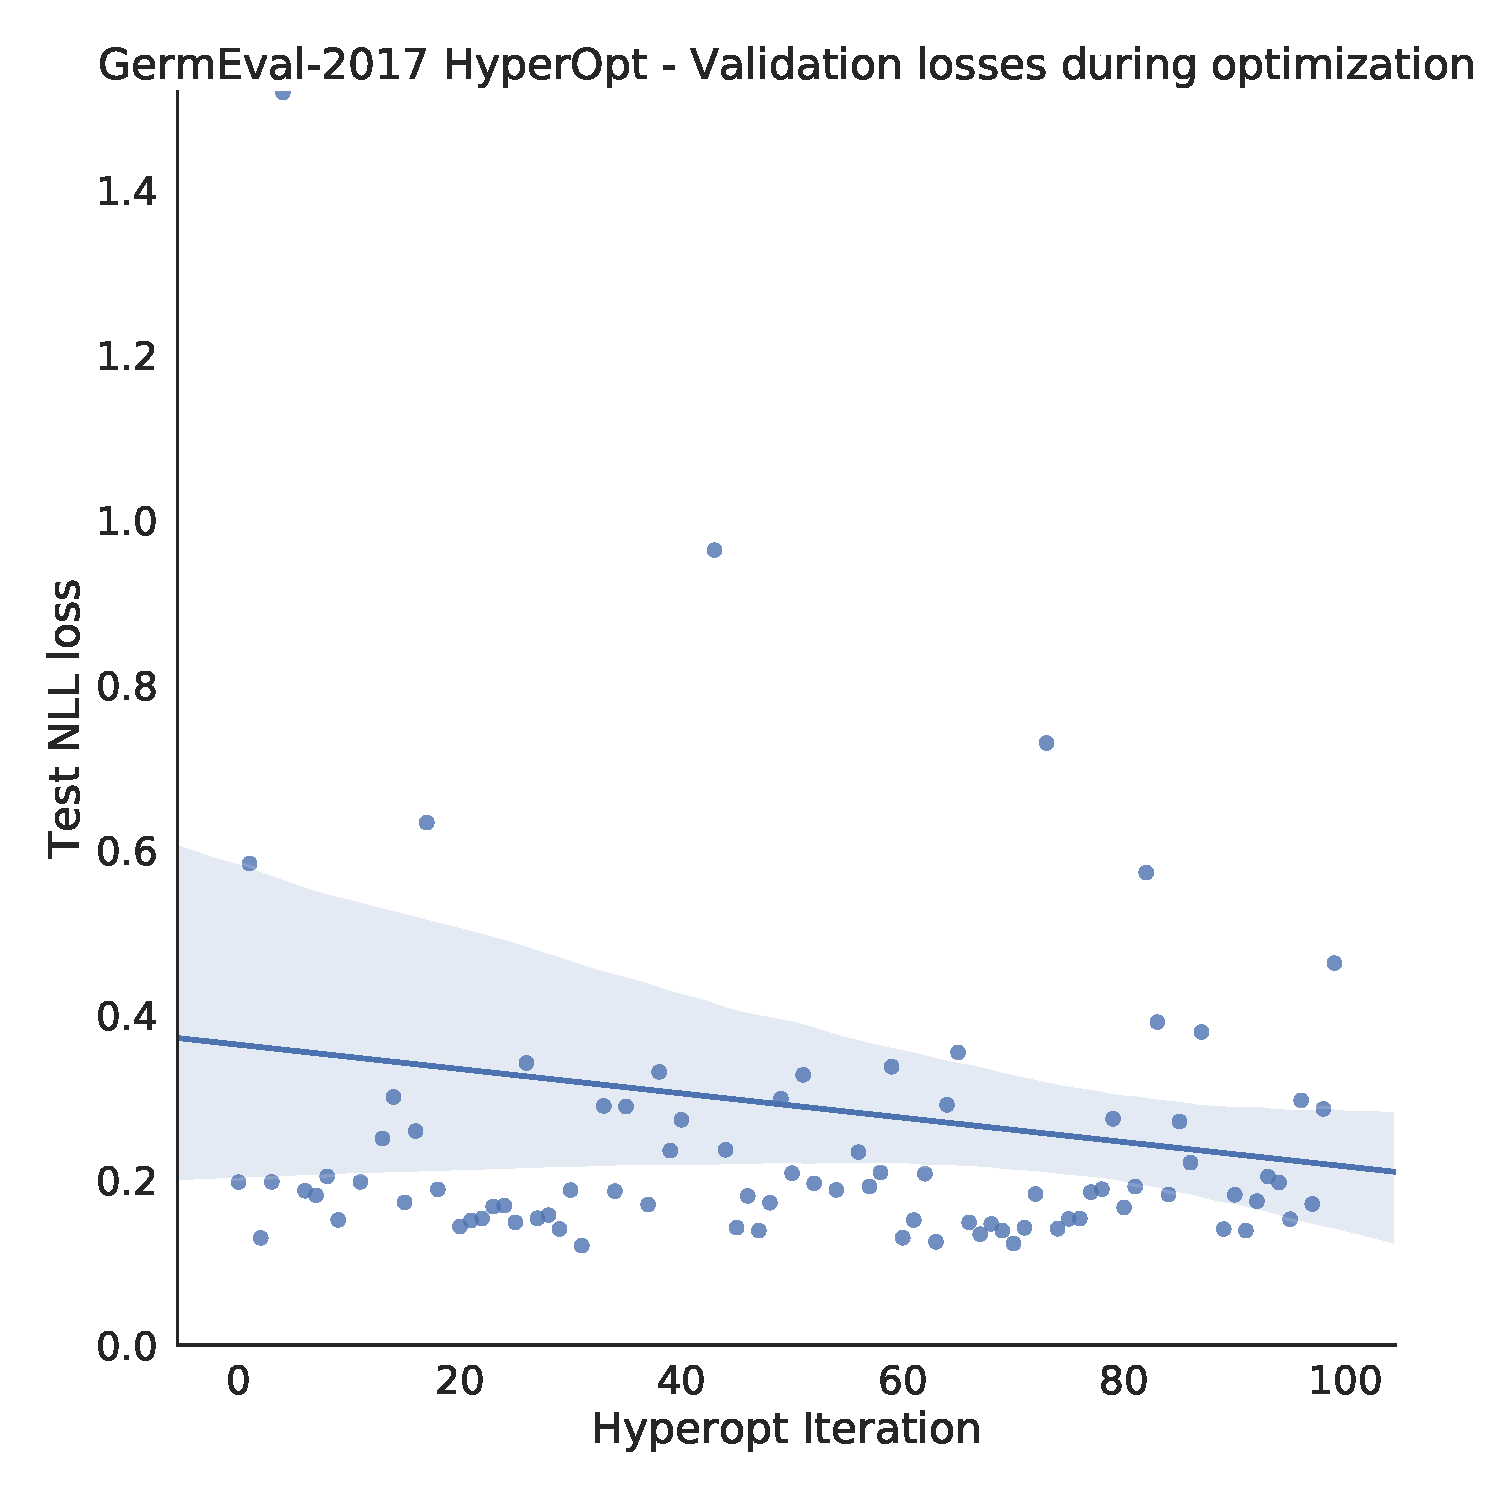
\includegraphics[width=0.49\textwidth]{figures/06_results/06_hp_ge_lm_loss-iteration_validation}
	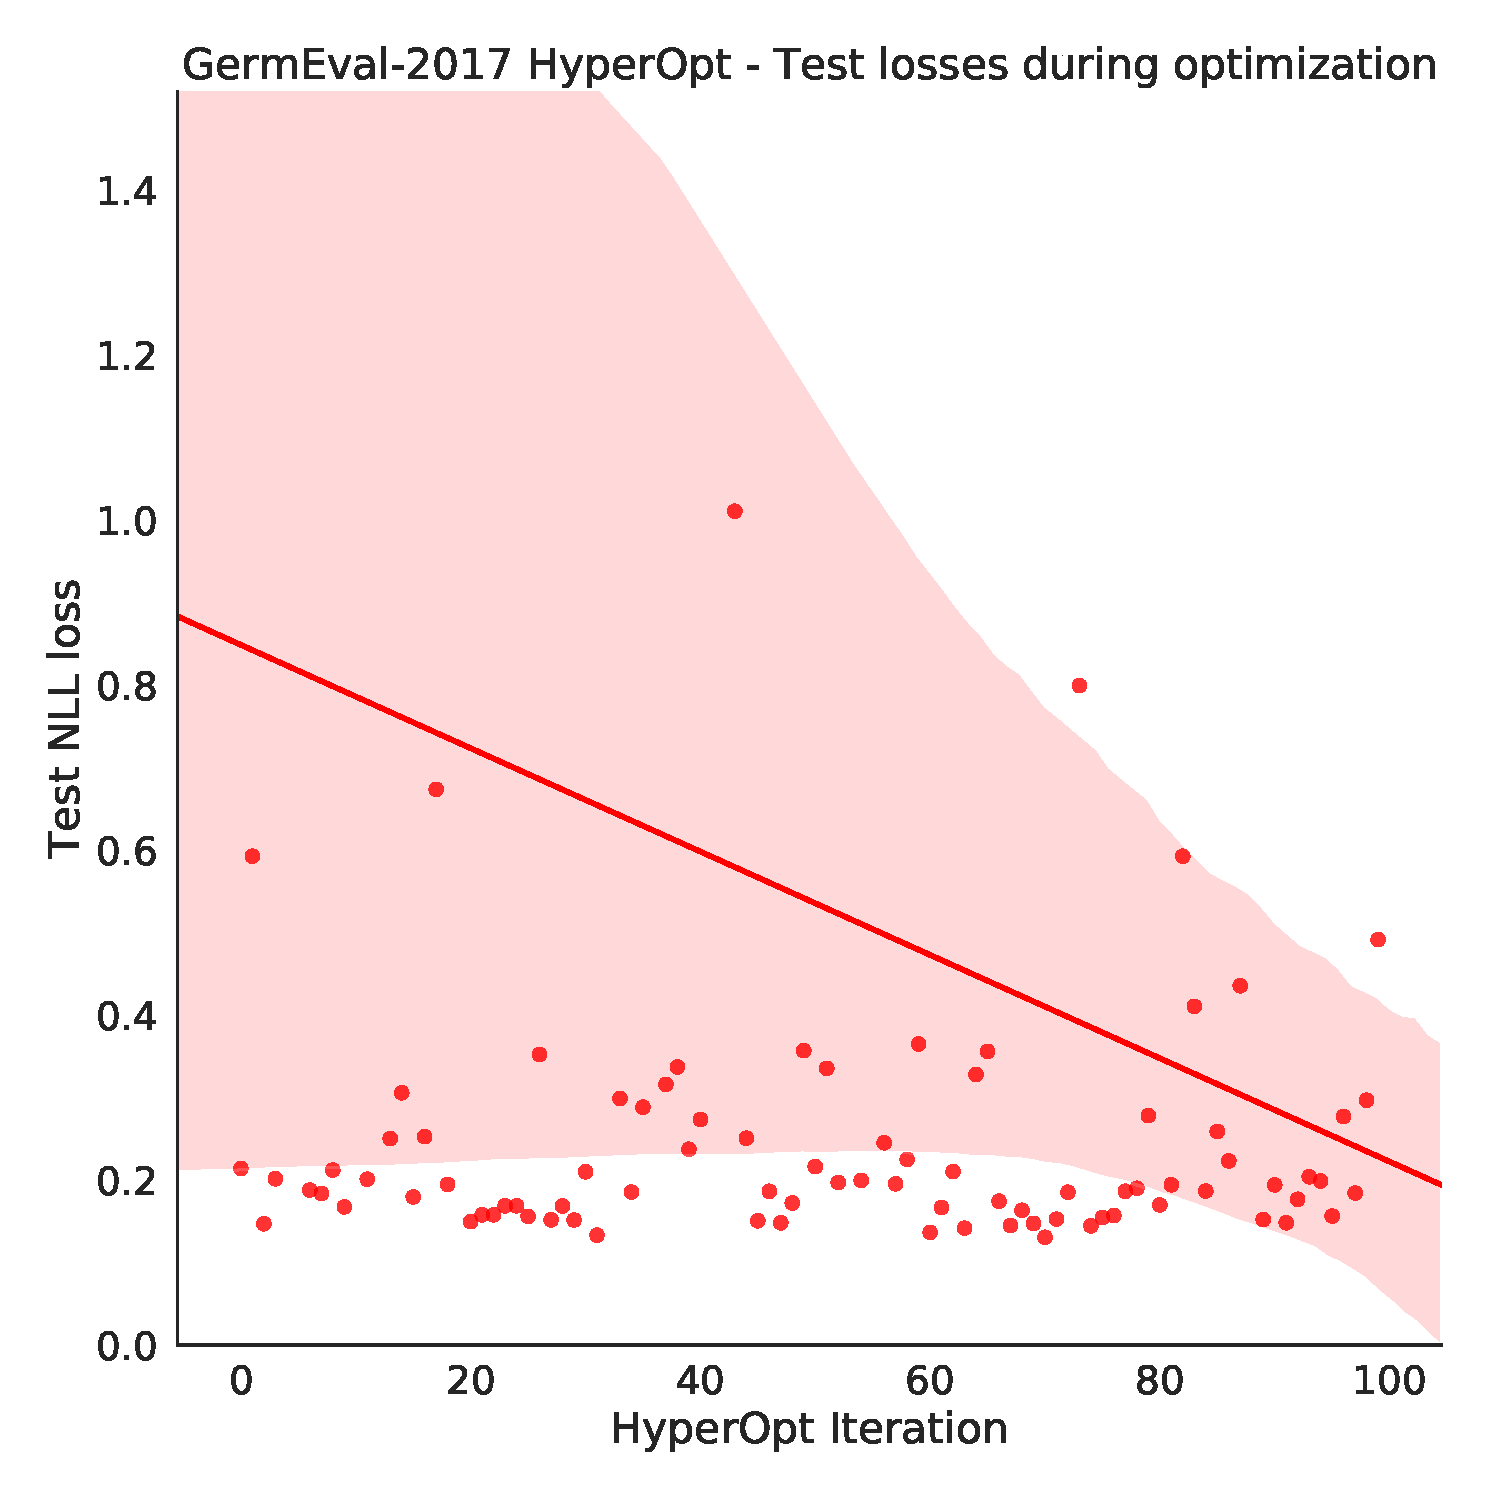
\includegraphics[width=0.49\textwidth]{figures/06_results/06_hp_ge_lm_loss-iteration_test}
	\caption{Validation- {(blue - left)} and test {(red - right)} losses during 100 Hyperopt iterations on GermEval-2017 dataset}
	\label{fig:06_ValidationLossGermEvalHp}
\end{figure}

To evaluate Hyperopt three evaluation runs with 100 iterations were performed.

\begin{enumerate}
	\item GermEval-2017 - \gls{tpe} on validation loss
	\item GermEval-2017 - Random search
	\item Organic Coarse Grained - \gls{tpe} on validation loss
\end{enumerate}

Figure \ref{fig:06_ValidationLossGermEvalHp} visualizes the improvement of the validation- and test losses on the GermEval-2017 dataset after 100 Hyperopt iterations. Is seems as if the regression line is negative in both cases which means that the \gls{tpe} algorithm Hyperopt uses suggests better results as the time moves on.

Unfortunately, the \gls{ols} analysis~\ref{tab:08_olsLossItVal} and~\ref{tab:08_olsLossItTest} in the appendix show that the negative correlation is in fact not significant. This implies that the \gls{tpe} algorithm does not sample parameters from the space which actually improve the loss of the model. This is even more obvious in figure~\ref{fig:06_F1GermEvalHp}. This figure shows the development of F1-Score during optimization. While the results on the left for GermEval might look like they improve over the course of the optimization the results\footnote{The improvement is still not significant {(0.340)}} for the optimization of the coarse organic dataset clearly show no improvement.
\medskip

There are several possible explanations which could contribute to this behaviour:

\begin{figure}[ht]
	\centering
	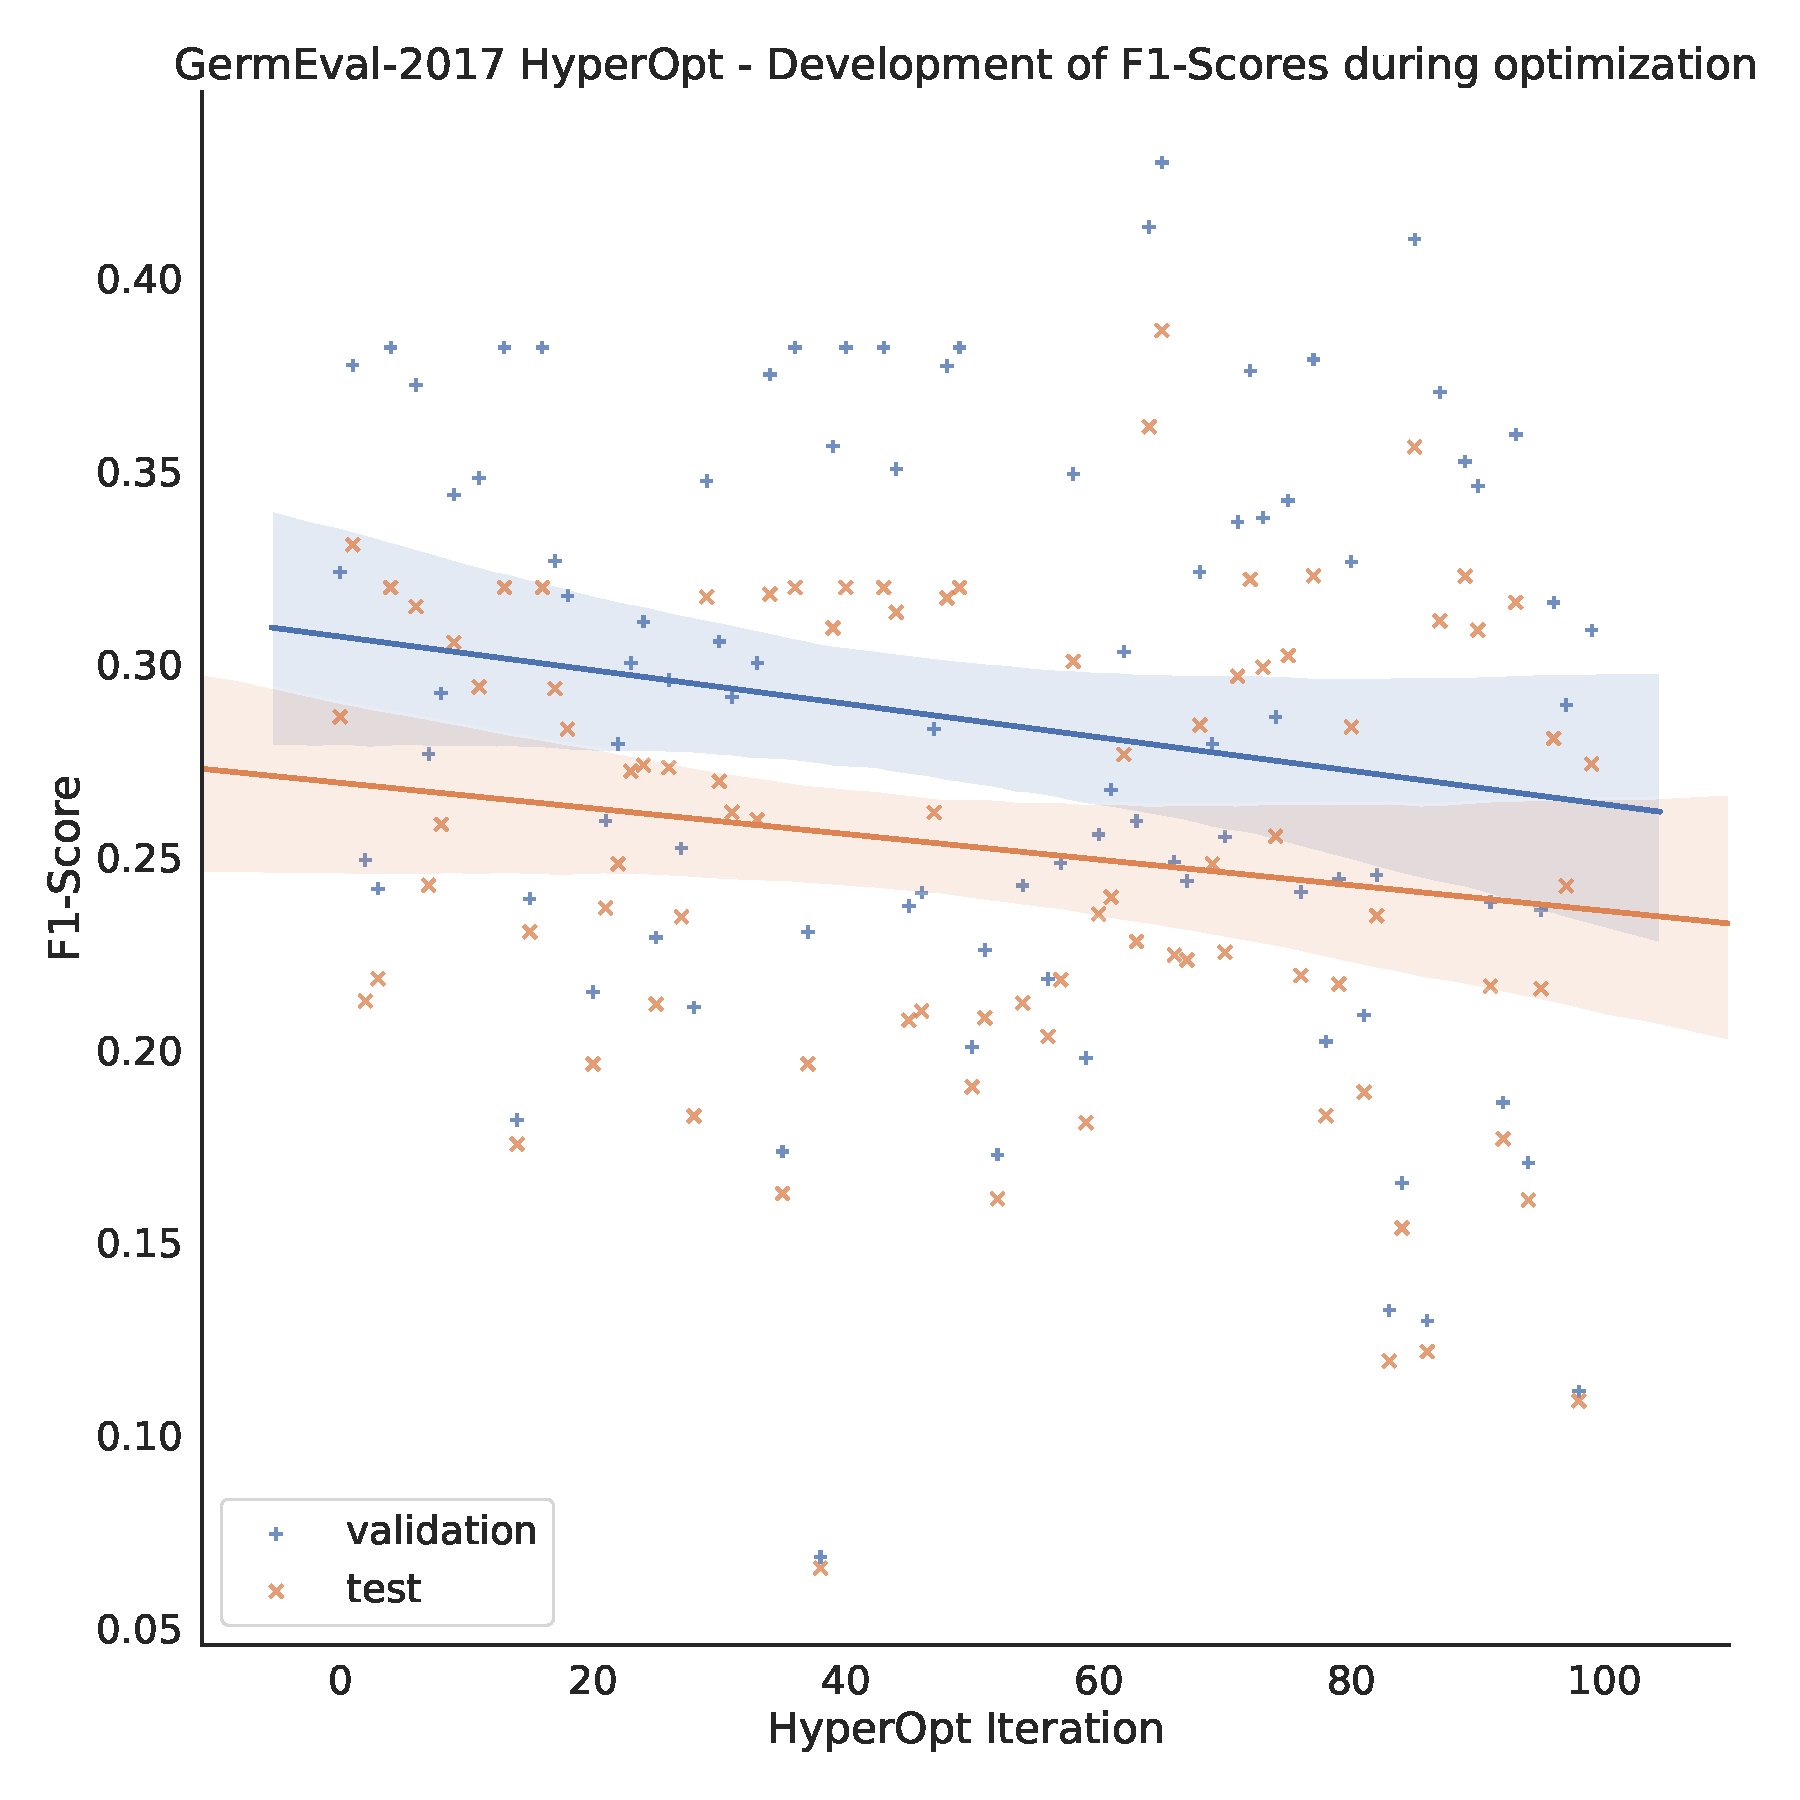
\includegraphics[width=0.49\textwidth]{figures/06_results/06_hp_ge_lm_f1time}
	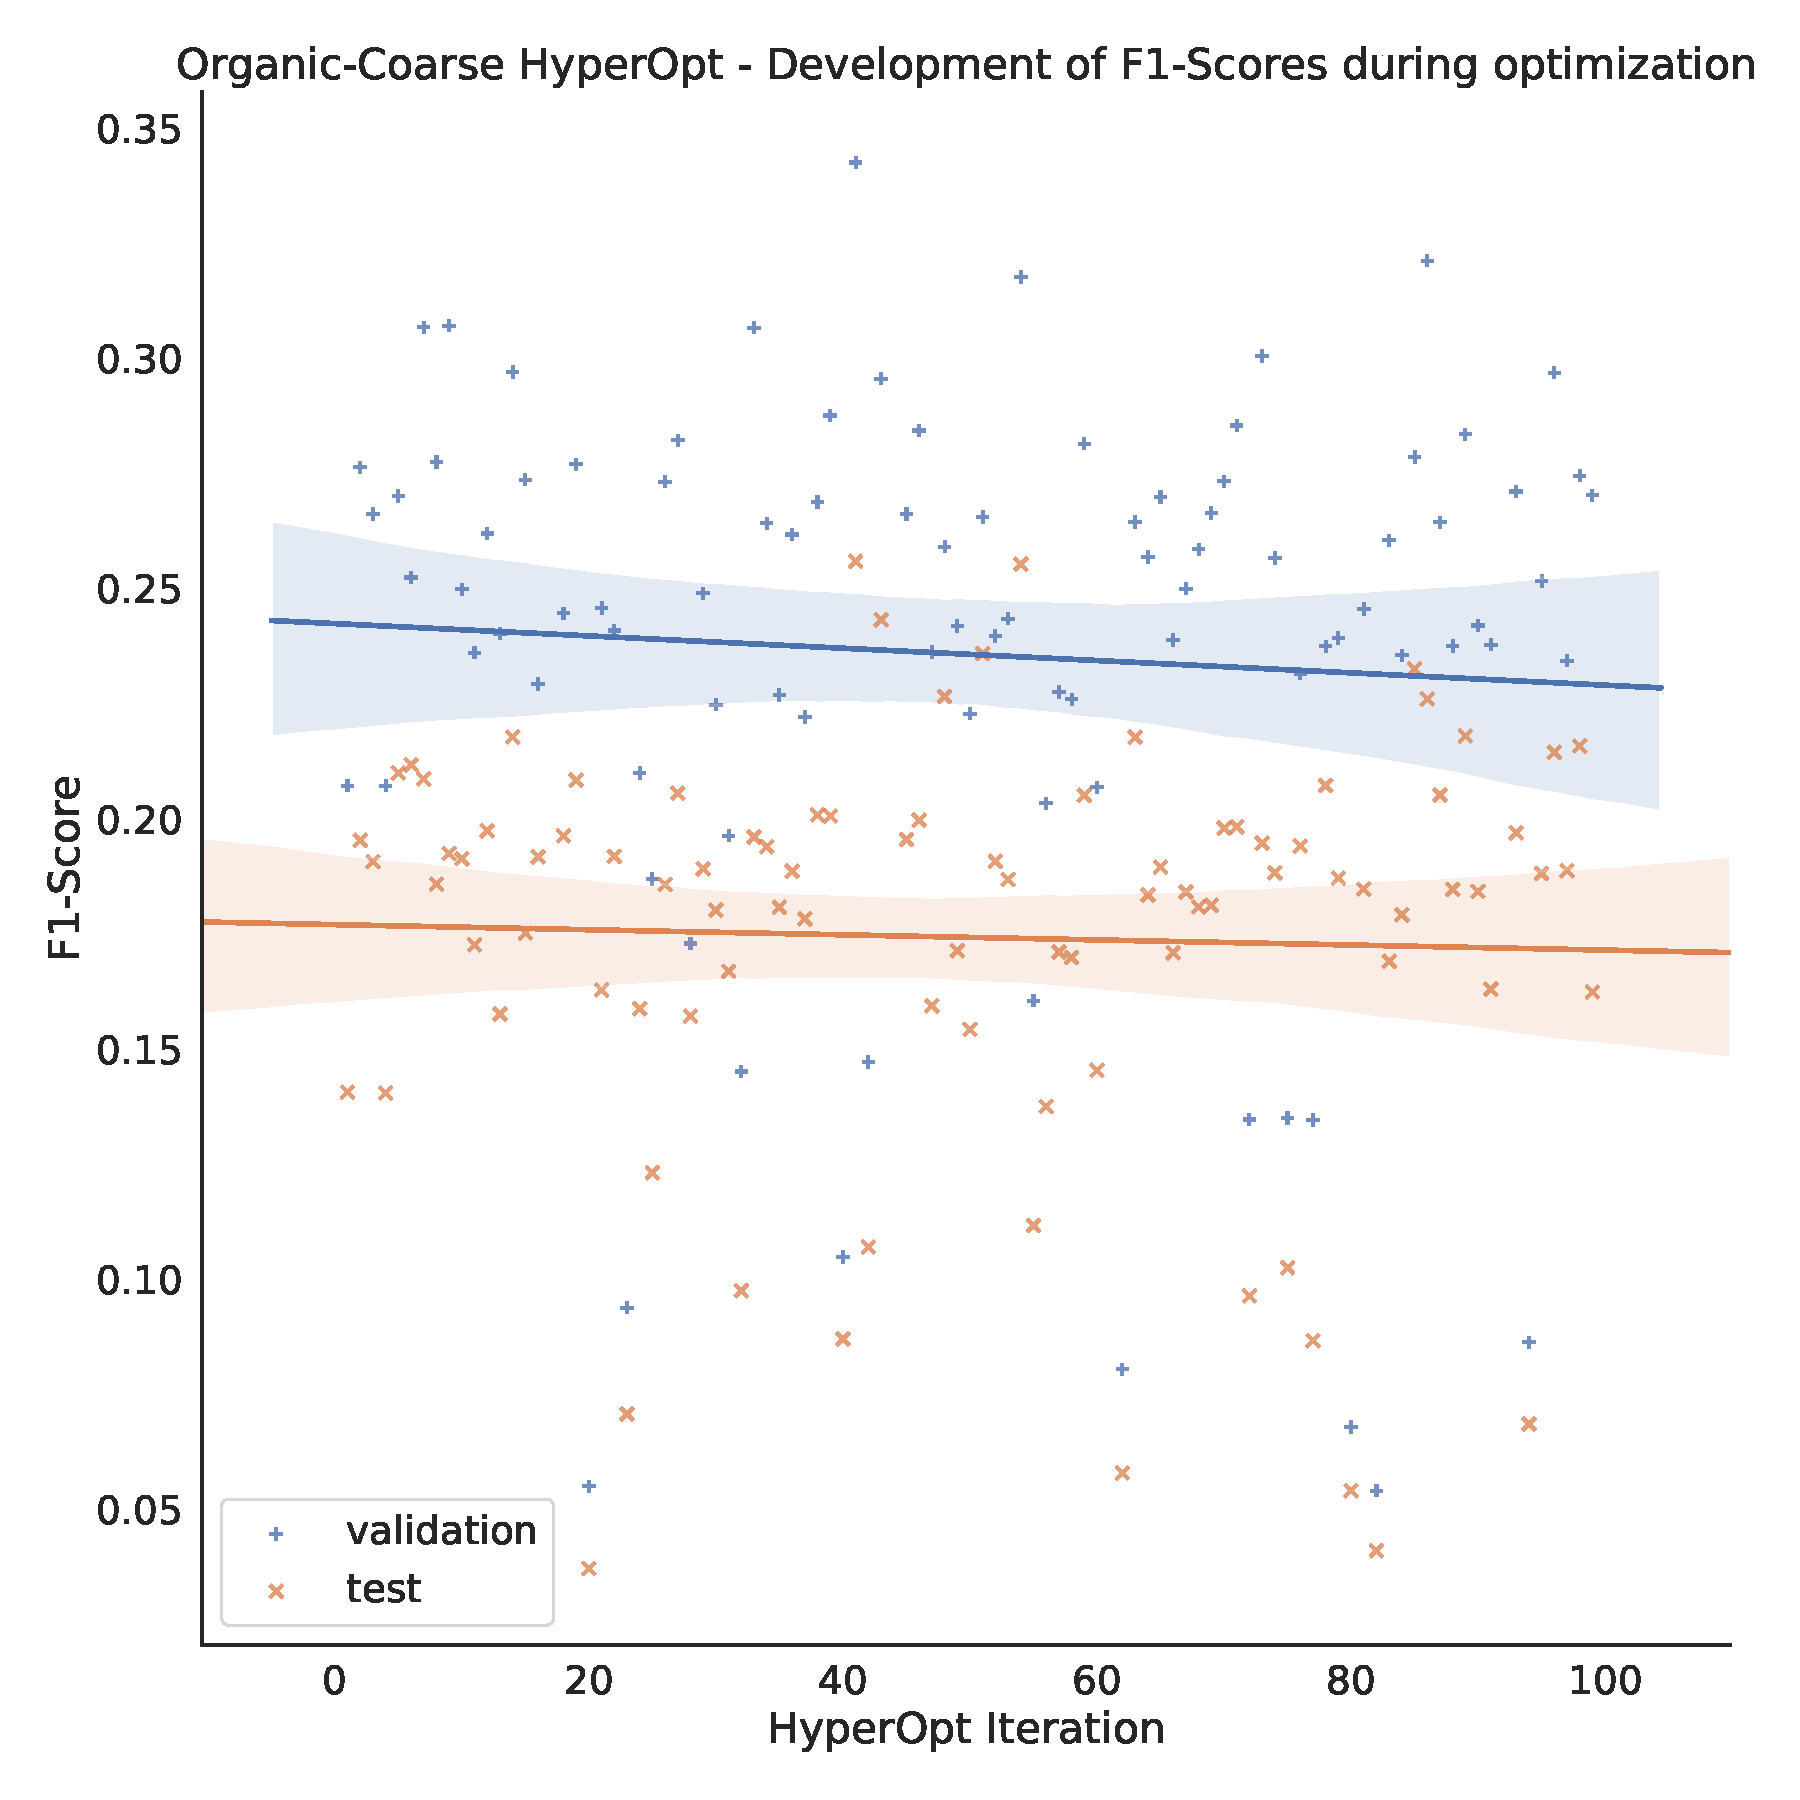
\includegraphics[width=0.49\textwidth]{figures/06_results/06_hp_og_lm_f1time}
	\caption{F1 Scores of the hyperparamter optimization of GermEval-2017 {(left)} and Coarse Organic 2019 datasets {(right)}.}
	\label{fig:06_F1GermEvalHp}
\end{figure}

\subsubsection*{Iterations}

First, it could be possible that 100 iterations are not enough to provide a stochastic model which is able to make good predictions in the hyperparameter space. It is worth noting that Bergstra et. al. show that hyperopt outperforms random search within 200 trials~\cite{Bergstra2013}. However, for most architectures it is not feasible to run an optimization search for much longer than 200 iterations let alone the 1000 iterations they claim as the point where hyperopt converges. 
\medskip

It is also worth mentioning that the Hyperopt module uses a random sampler for the first 10 iterations to get data points to initialize the \glspl{tpe}. Decreasing this number could yield to better results for computational expensive models since the algorithm is forced to suggest values earlier.

\subsubsection*{Hyperparamter Search Space}

It is possible that the hyperparameter search space which Hyperopt uses to generate new parameters is too large. Table \ref{tab:08_hpSpace} shows the hyperparameter search space for the optimization of the GermEval-2017 dataset. There are parameters which do not change the outcome by a huge margin and then there are parameters which decide whether or not the model trains at all. However, finding those parameters is a challenging task.

\subsubsection*{Warmup Phase}
\label{sec:06_hp_warmup}
\begin{table}[]
	\centering
	\begin{tabular}{lrrrrr}
	\multicolumn{6}{c}{GermEval-2017} \\

	\toprule
	{} &  count &      mean &       std &       min &       max \\
	Aspect Head &        &           &           &           &           \\
	\midrule
	\multicolumn{6}{c}{Warmup Iterations 1 - 10*} \\
	CNN-A    &    6 &  0.267644 &  0.050316 &  0.212655 &  0.330922 \\
	MLS-A    &    3 &  0.294608 &  0.032134 &  0.258432 &  0.319838 \\
	\midrule
	\multicolumn{6}{c}{\gls{tpe} Iterations 1 - 100} \\
	CNN-A    &   67 &  0.249094 &  0.066835 &  0.065565 &  0.386465 \\
	MLS-A    &   23 &  0.261533 &  0.044603 &  0.181078 &  0.356296 \\
	\bottomrule
	\end{tabular}
	\caption{Result of sampling of Aspect Head choices during \gls{tpe} Hyperopt optimization. Values show micro F1-score achieved by models on the GermEval-2017 dataset. * The 10th iteration failed which is the reason why the warmup does not sum up to 10.}
	\label{tab:08_hpAspectHeadsSpace}	
\end{table}

\gls{tpe} supports tree structures for the search space. In the search space used for the optimization there is one tree-like parameter which is the choice of the aspect head architecture. \gls{tpe} can either choose a \gls{mlsa} or a \gls{cnna}. The \gls{mlsa} does not have additional parameter nodes, whereas the \gls{cnna} has 4 additional parameters.
\medskip

\gls{mlsa} has a higher mean F1-score of 0.263 compared to \gls{cnna} which achieves 0.250. Despite the higher mean score, \gls{tpe} only sampled \gls{mlsa} 23 times compared to 67 times.

This becomes even more interesting when looking at the \gls{tpe} warmup phase. During warmup, \gls{mlsa} is chosen 3 times and \gls{cnna} is chosen 6 times. This is roughly the same distribution compared to the later \gls{tpe} iterations. 

For greater detail refer to table~\ref{tab:08_hpAspectHeadsSpace}. There is also a violinplot which visualizes the impact of the aspect head choice in the appendix as figure \ref{fig:06_ge_aspectHeadChoices}.
\medskip

In contrast, during the warmup phase of the hyperopt run on the coarse organic dataset, Hyperopt sampled \gls{cnna} 2 times and \gls{mlsa} 7 times which is exactly the other way around. During the \gls{tpe} iterations, \gls{cnna} was sampled 14- and \gls{mlsa} 71 times. Again, this is the exact opposite of the previous optimization on the GermEval-2017 dataset.
\medskip

This leads to the following conclusion: During the warmup phase of Hyperopt the search space is randomly sampled. This random sampling distribution is adhered to during the whole \gls{tpe} suggestion phase. This leads to results which are heavily dependent on the first 10 random iterations.

\subsubsection*{Comparison with a Random Search}

\begin{figure}[ht]
	\centering
	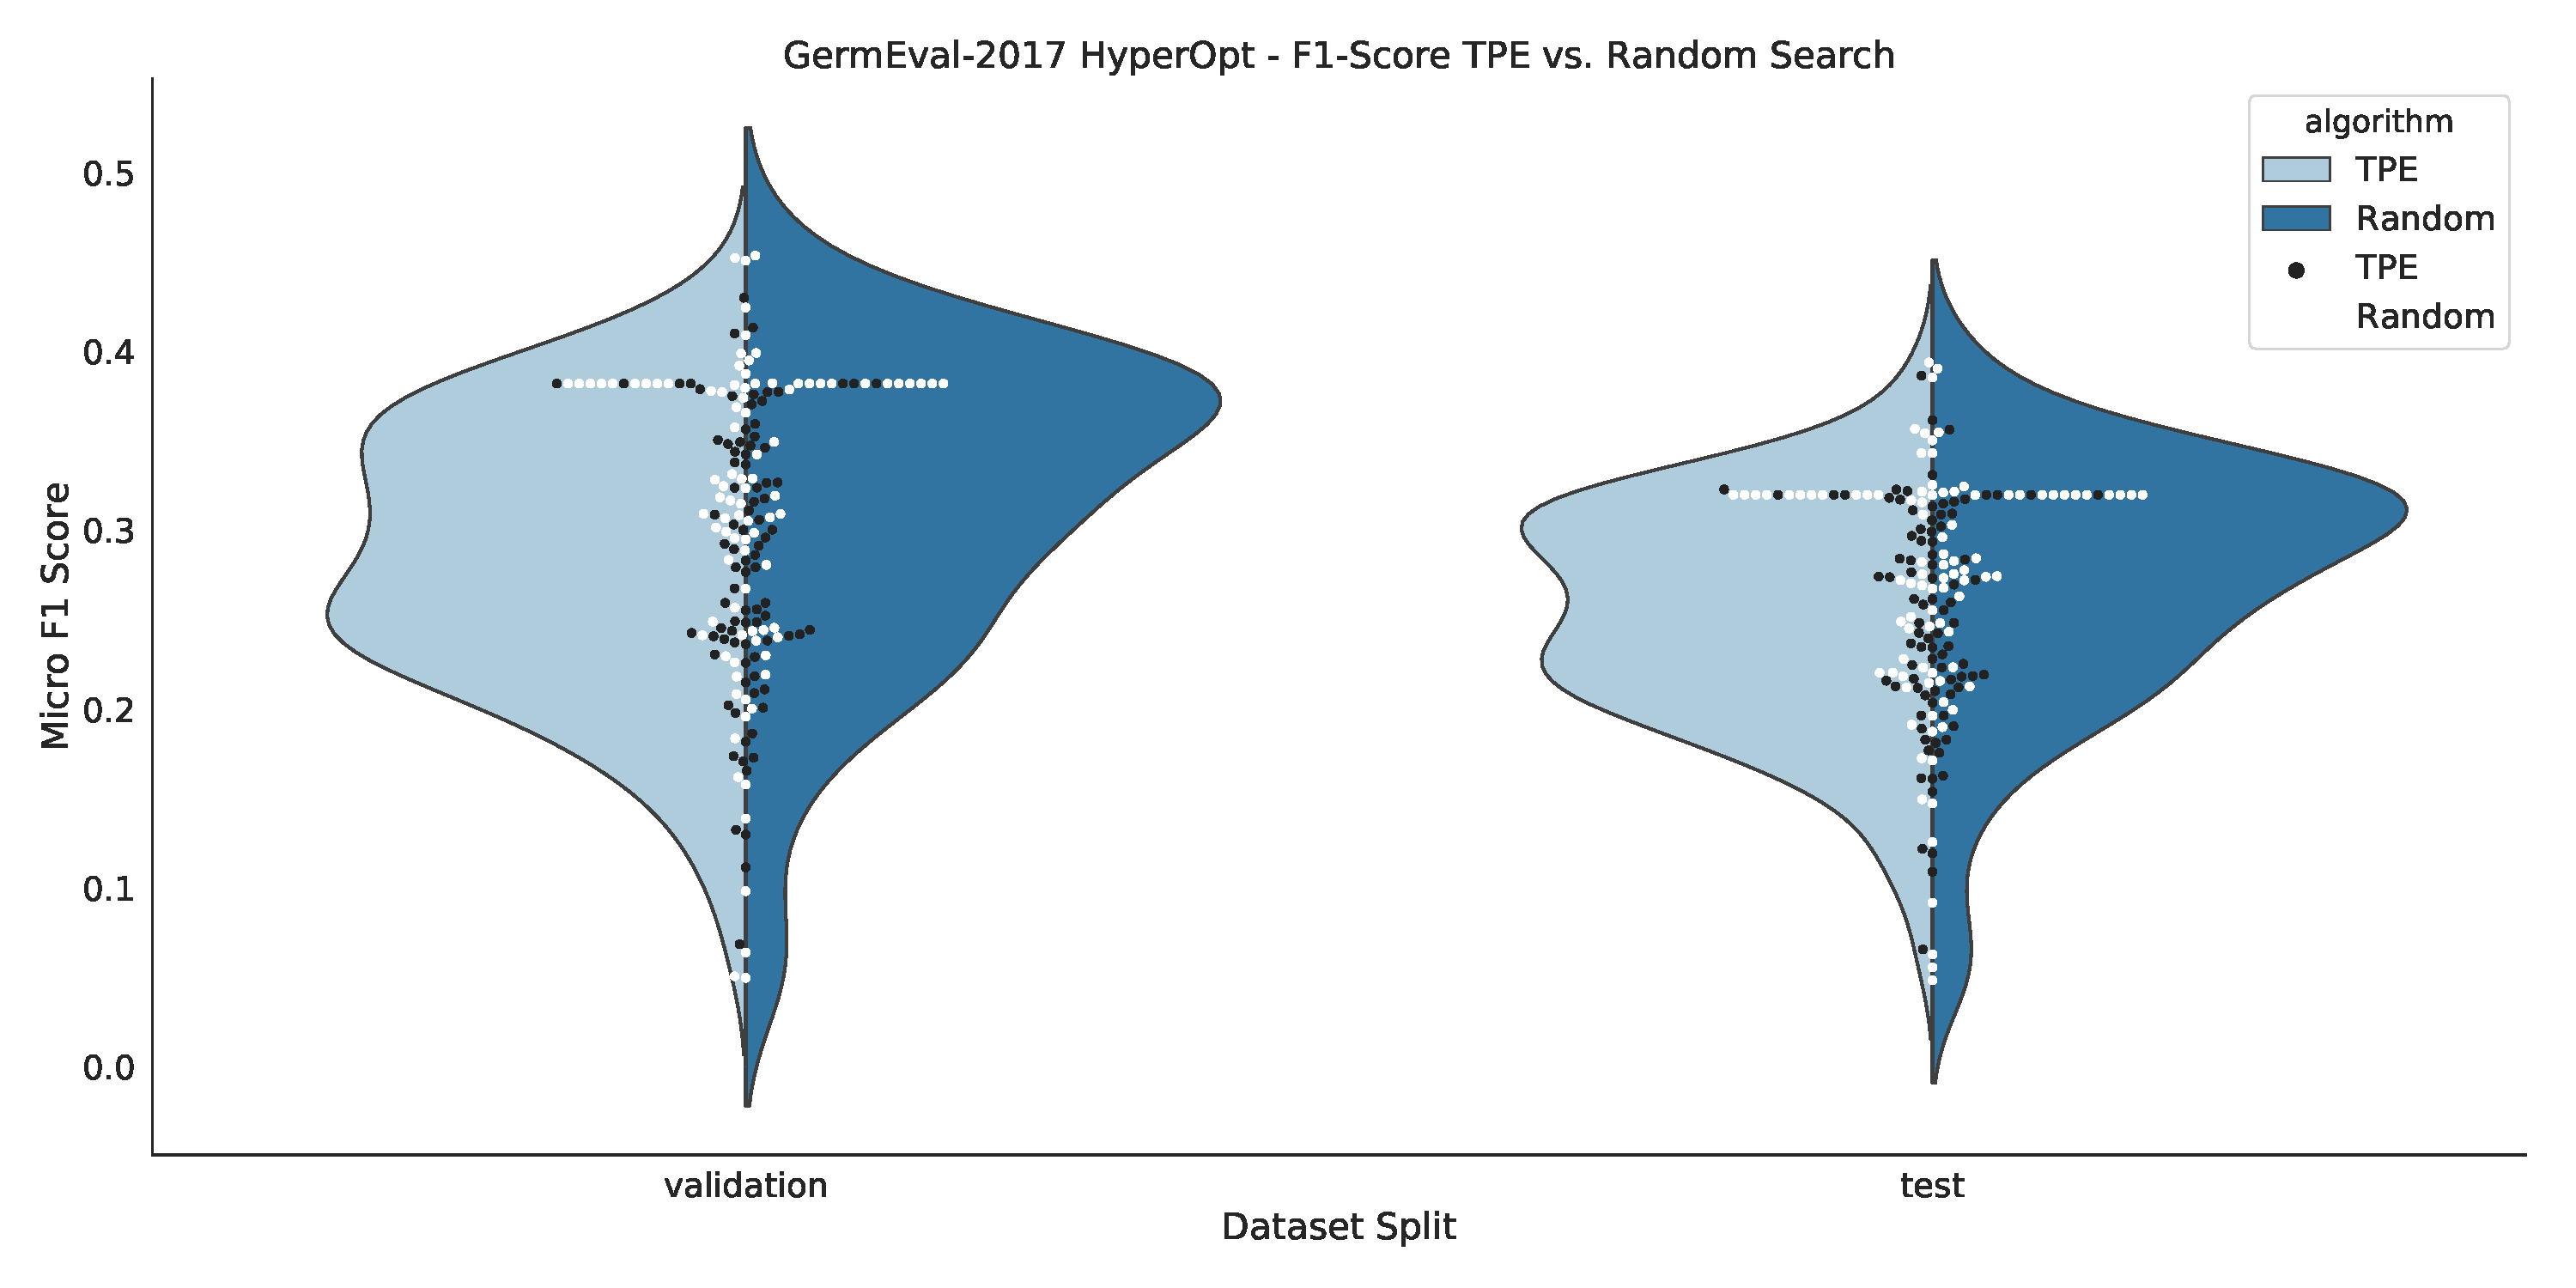
\includegraphics[width=\textwidth]{figures/06_results/06_hp_ge_vio_tpeRand}
	\caption{Comparison of HyperOpt TPE algorithm against a classical random search. The results for TPE are light blue on the left, whereas results for the random search are a deep blue on the right.}
	\label{fig:06_HpOptimTpe_Rand}
\end{figure}

To confirm the findings above a completely random search was performed by Hyperopt on the same number of iterations. The result of this comparison is plotted in figure~\ref{fig:06_HpOptimTpe_Rand}. This violinplot visualizes the result of both optimization runs. The light blue density curve on the left shows the F1 scores from the \gls{tpe} generated models. A wider body on the density curve means that more observations for this particular score value were recorded at this part. The black dots correspond to the actual individual F1-Score observations. The dark blue parts and the white dots correspond to the F1-scores which originated by randomly generated hyperparameters.

\subsection{Model Parameters}

Due to the high dimensionality of the hyperparameter search space, statistical significance tests will not show any significant correlations between the parameter and an improvement of the F1-Score. For each single parameter change, all other parameters will also change and they influence the model as well. While not possible to evaluate the results with statistical significance it is possible to derive certain assumptions from the data which will be discussed in the following sections.

\subsubsection{Aspect Heads}

As discussed in section~\ref{sec:06_hp_warmup} it is not entirely possible to favor one or the other aspect head. Both can provide similar results. 

\begin{figure}[ht]
	\centering
	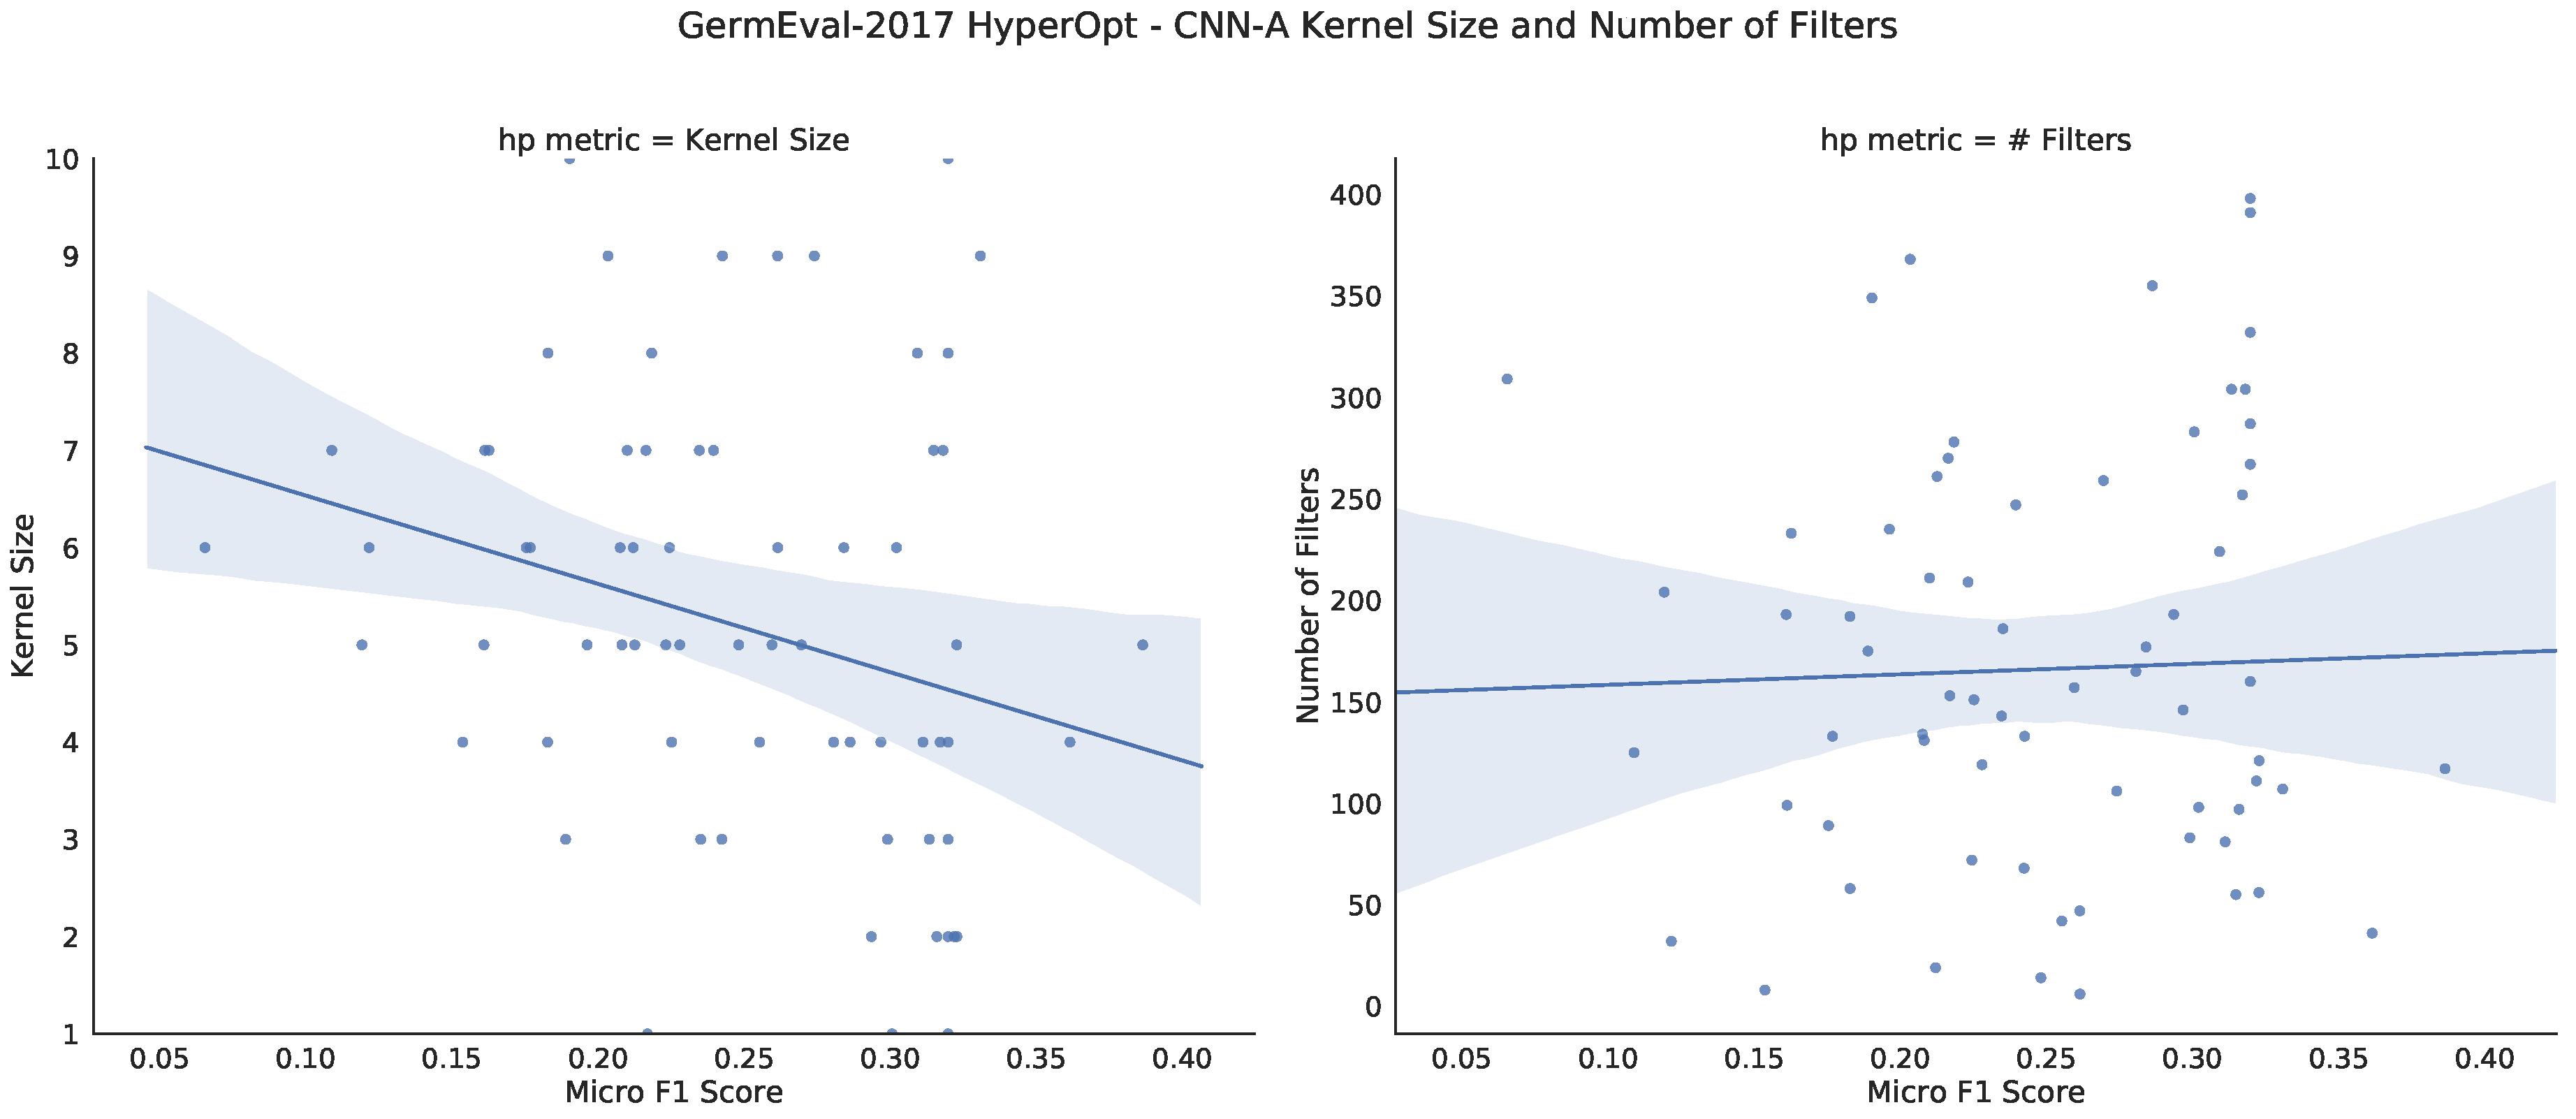
\includegraphics[width=\textwidth]{figures/06_results/06_hp_ge_lm_cnnParams_test}
	\caption{Impact of CNN parameters on micro F1-score. The graph on the left shows the impact of the kernel size on the model performance. The graph on the right depicts the influence of the number of filters on the F1-score.}
	\label{fig:06_HpOptim_CnnParams}
\end{figure}

Figure~\ref{fig:06_HpOptim_CnnParams} shows the impact of the two \gls{cnna} parameters 'Kernel Size' and 'Number of Filters'. The number of filters does not seem to impact the result. However, there is a {(statistical\footnote{Significant at a $p$-value of 0.05})} significant negative correlation between the kernel size and the model performance. 

Smaller filters lead to a performance improvement compared to bigger filters. This result seems to follow the literature. For instance, Schmitt et. al. use filter sizes of 3, 4 and 5~\cite{Schmitt2018}.
\medskip

There is no significant change for the other two parameters 'Kernel Padding' and 'Kernel Stride'. The impact on the F1-Score of both parameters is visualized in figure~\ref{fig:06_HpOptim_CnnParams2} in the appendix.

\subsubsection{Point-wise Feed-Forward Layer Size}

In the original transformer model the inner \acrfull{pwfc} has a dimensionality of 1024 while the model size has a dimensionality of 512~\cite{Vaswani2017c}. This is a 2x increase over the model size. Due to the availability of pretrained Glove or Fasttext embeddings our \gls{absat} model only uses a model size of 300. Consequently, the inner \gls{pwfc} layer dimensionality should be around 600. However, layer sizes above 300-400 neurons quickly lead to interesting model behavior. After a few training iterations the \glspl{pwfc} transform every input to the exact same output. In other words, no matter what the model gets as input it always predicts the same output.
\medskip

The solution for this overfitting behavior is to use a smaller inner \gls{pwfc}. Values from 100 to 200 neurons lead to the best results.

This is extremely interesting since it completely changes the task of the \glspl{pwfc}. From a layer with a higher dimensionality than the model to a bottleneck layer with a lower dimensionality. A bigger layer may allow for more complex and expressive features to be learned while a smaller bottleneck layer limits the expressiveness and forces the network to focus on crucial features~\cite{Ramsundar2015}.

\subsection{Data Preprocessing}
\label{subsec:06_dataPreprocessing}
In the following section we discuss the impact of the preprocessing steps and how they affect the overall model performance. 

\begin{figure}
	\centering
	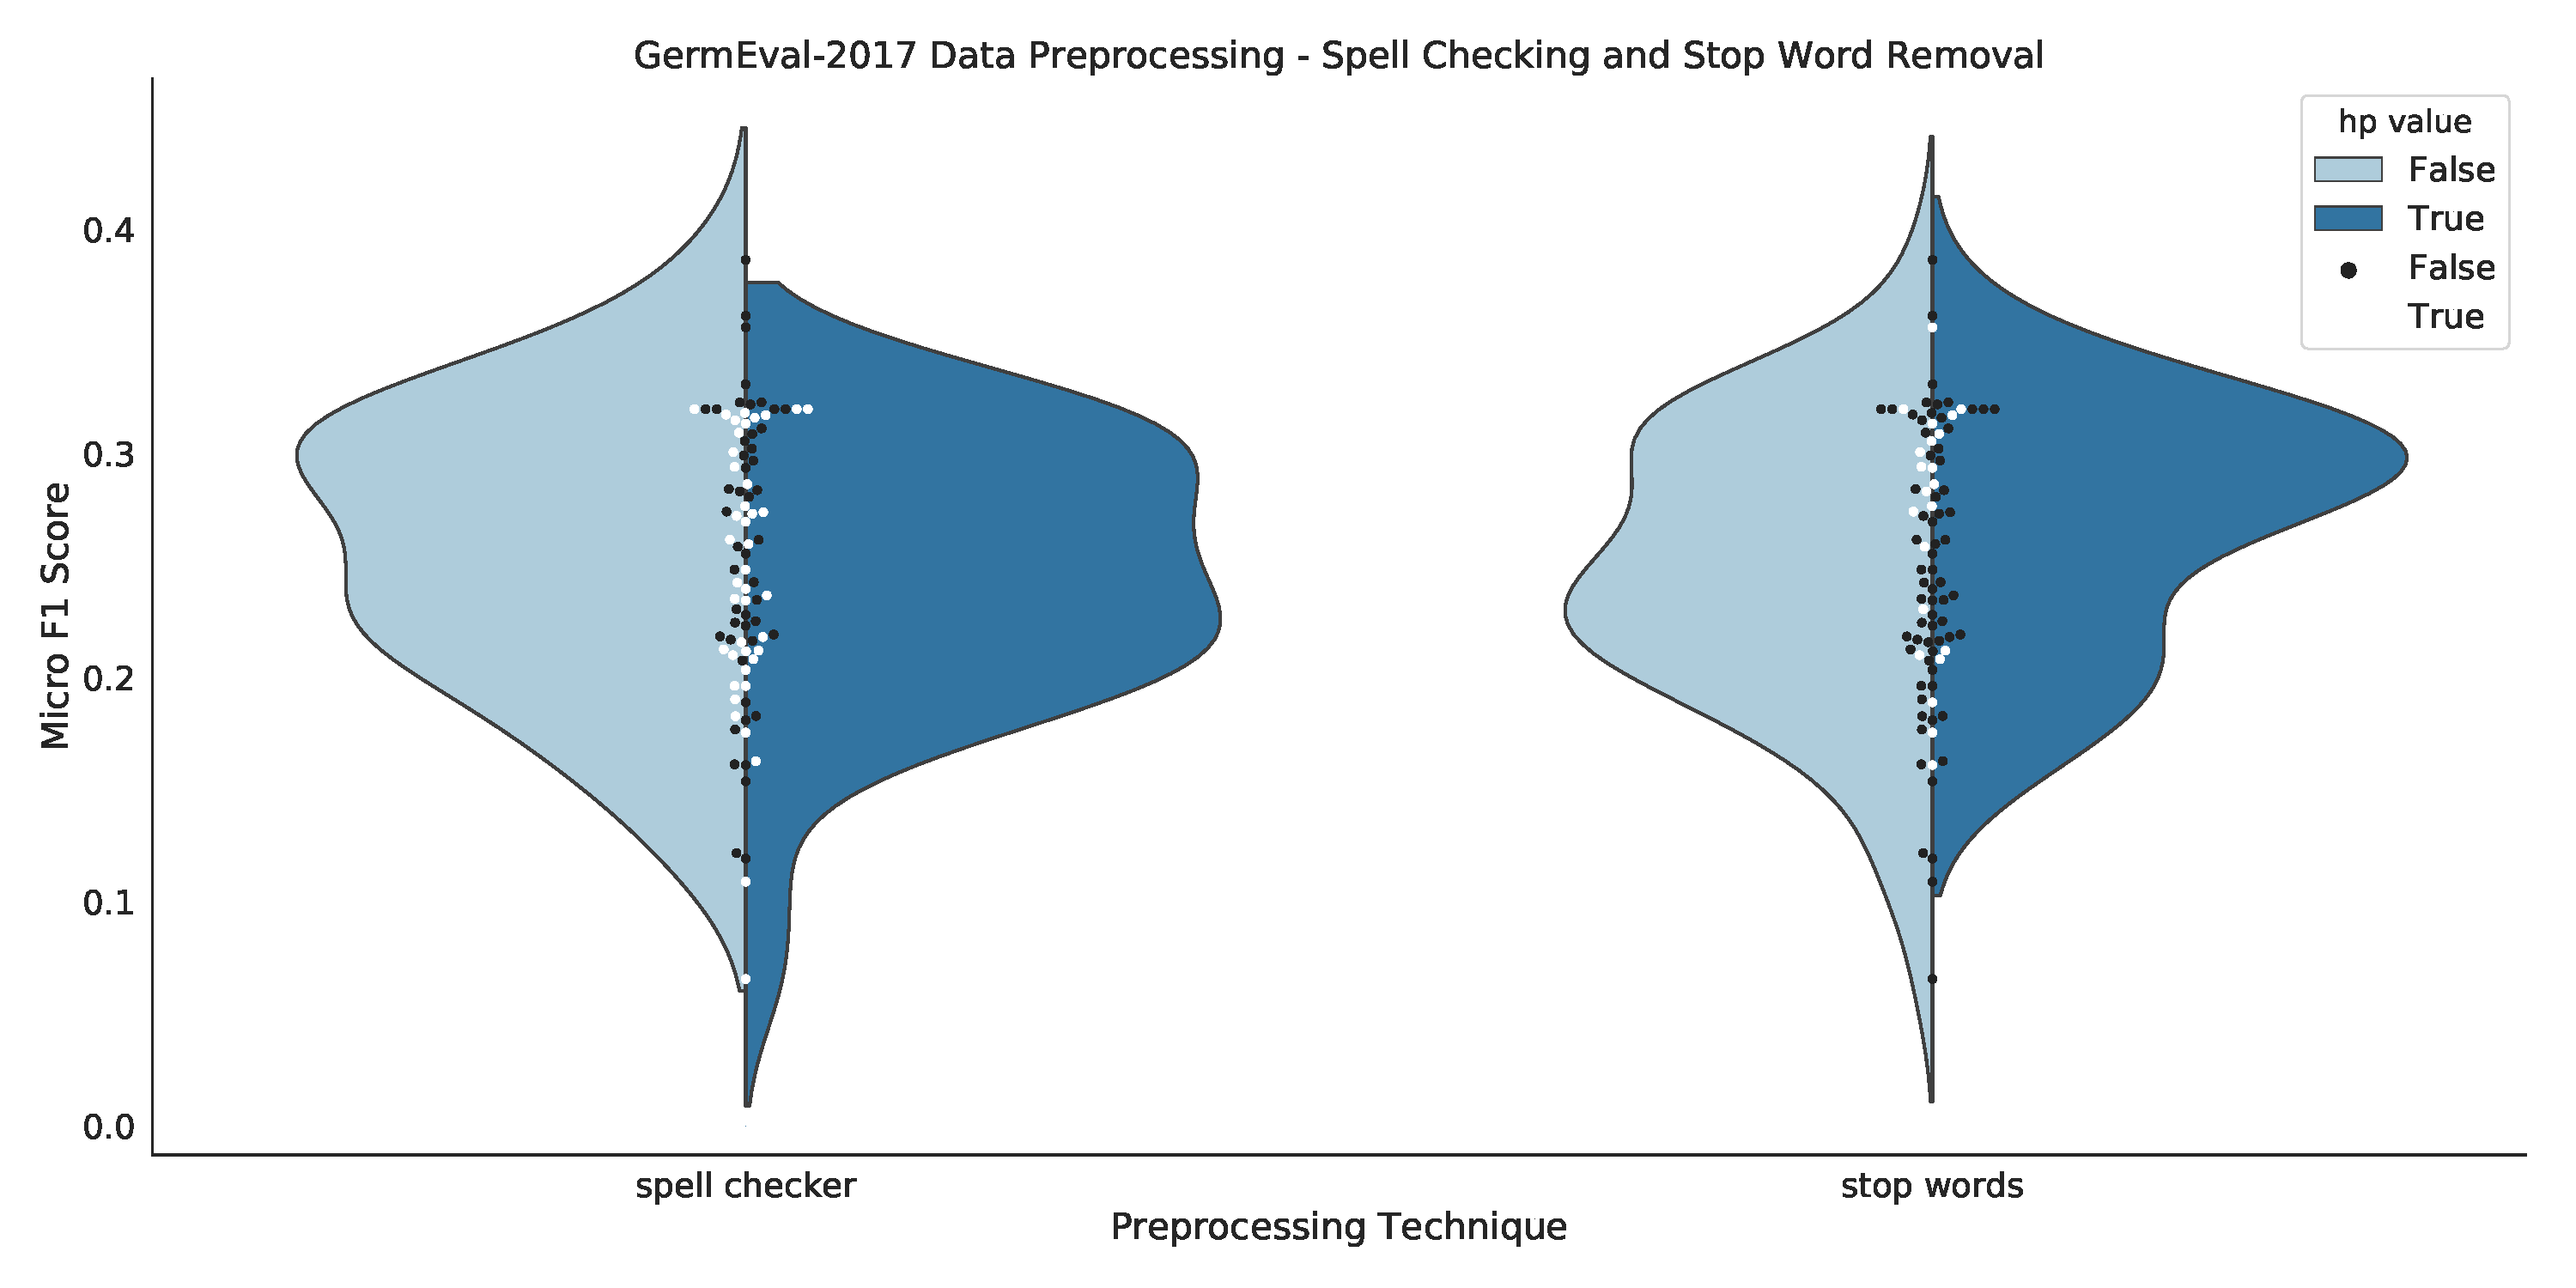
\includegraphics[width=\textwidth]{figures/06_results/06_hp_ge_vio_data}
	\caption{Comparison of preprocessing techniques - Impact of Spell checking and Stop Word Removal on Validation Micro F1-Score}
	\label{fig:06_PreprocessingHp}
\end{figure}

\subsubsection{Spell Checking}

The left side of figure~\ref{fig:06_PreprocessingHp} shows the impact of spell checking on the GermEval-2017 dataset. In this instance, spell checking negatively impacted the performance of the classifier. There are a few explanations for this performance.
\medskip

Social media content contains a lot of special characters and words which are not part of a regular dictionary. However, especially those words might carry the most sentiment. By replacing those words it is possible that a lot of information is lost.
\medskip

Tweets and forums posts about travel contain a lot of special abbreviations that spell checkers do not recognize. Persons might be talking about the bad performance of the public transport operator \gls{mvg} but the spell checker replaces 'MVG' with 'mag' which changes the sentence dramatically.

\subsubsection{Stop Word Removal}

Stop words are a group of words which are very common in a language but carry little actual information. Examples for stop words are 'the', 'is' or 'what'. The results for stop word removal is shown in figure~\ref{fig:06_PreprocessingHp} on the right side for GermEval-2017. In this specific instance, removing them improves performance. However, this was not as clear for the organic dataset where removing stop words did not significantly improve the performance.

\subsubsection{Comment Clipping}
\label{subsec:06_CommentClipping}

\begin{figure}
	\centering
	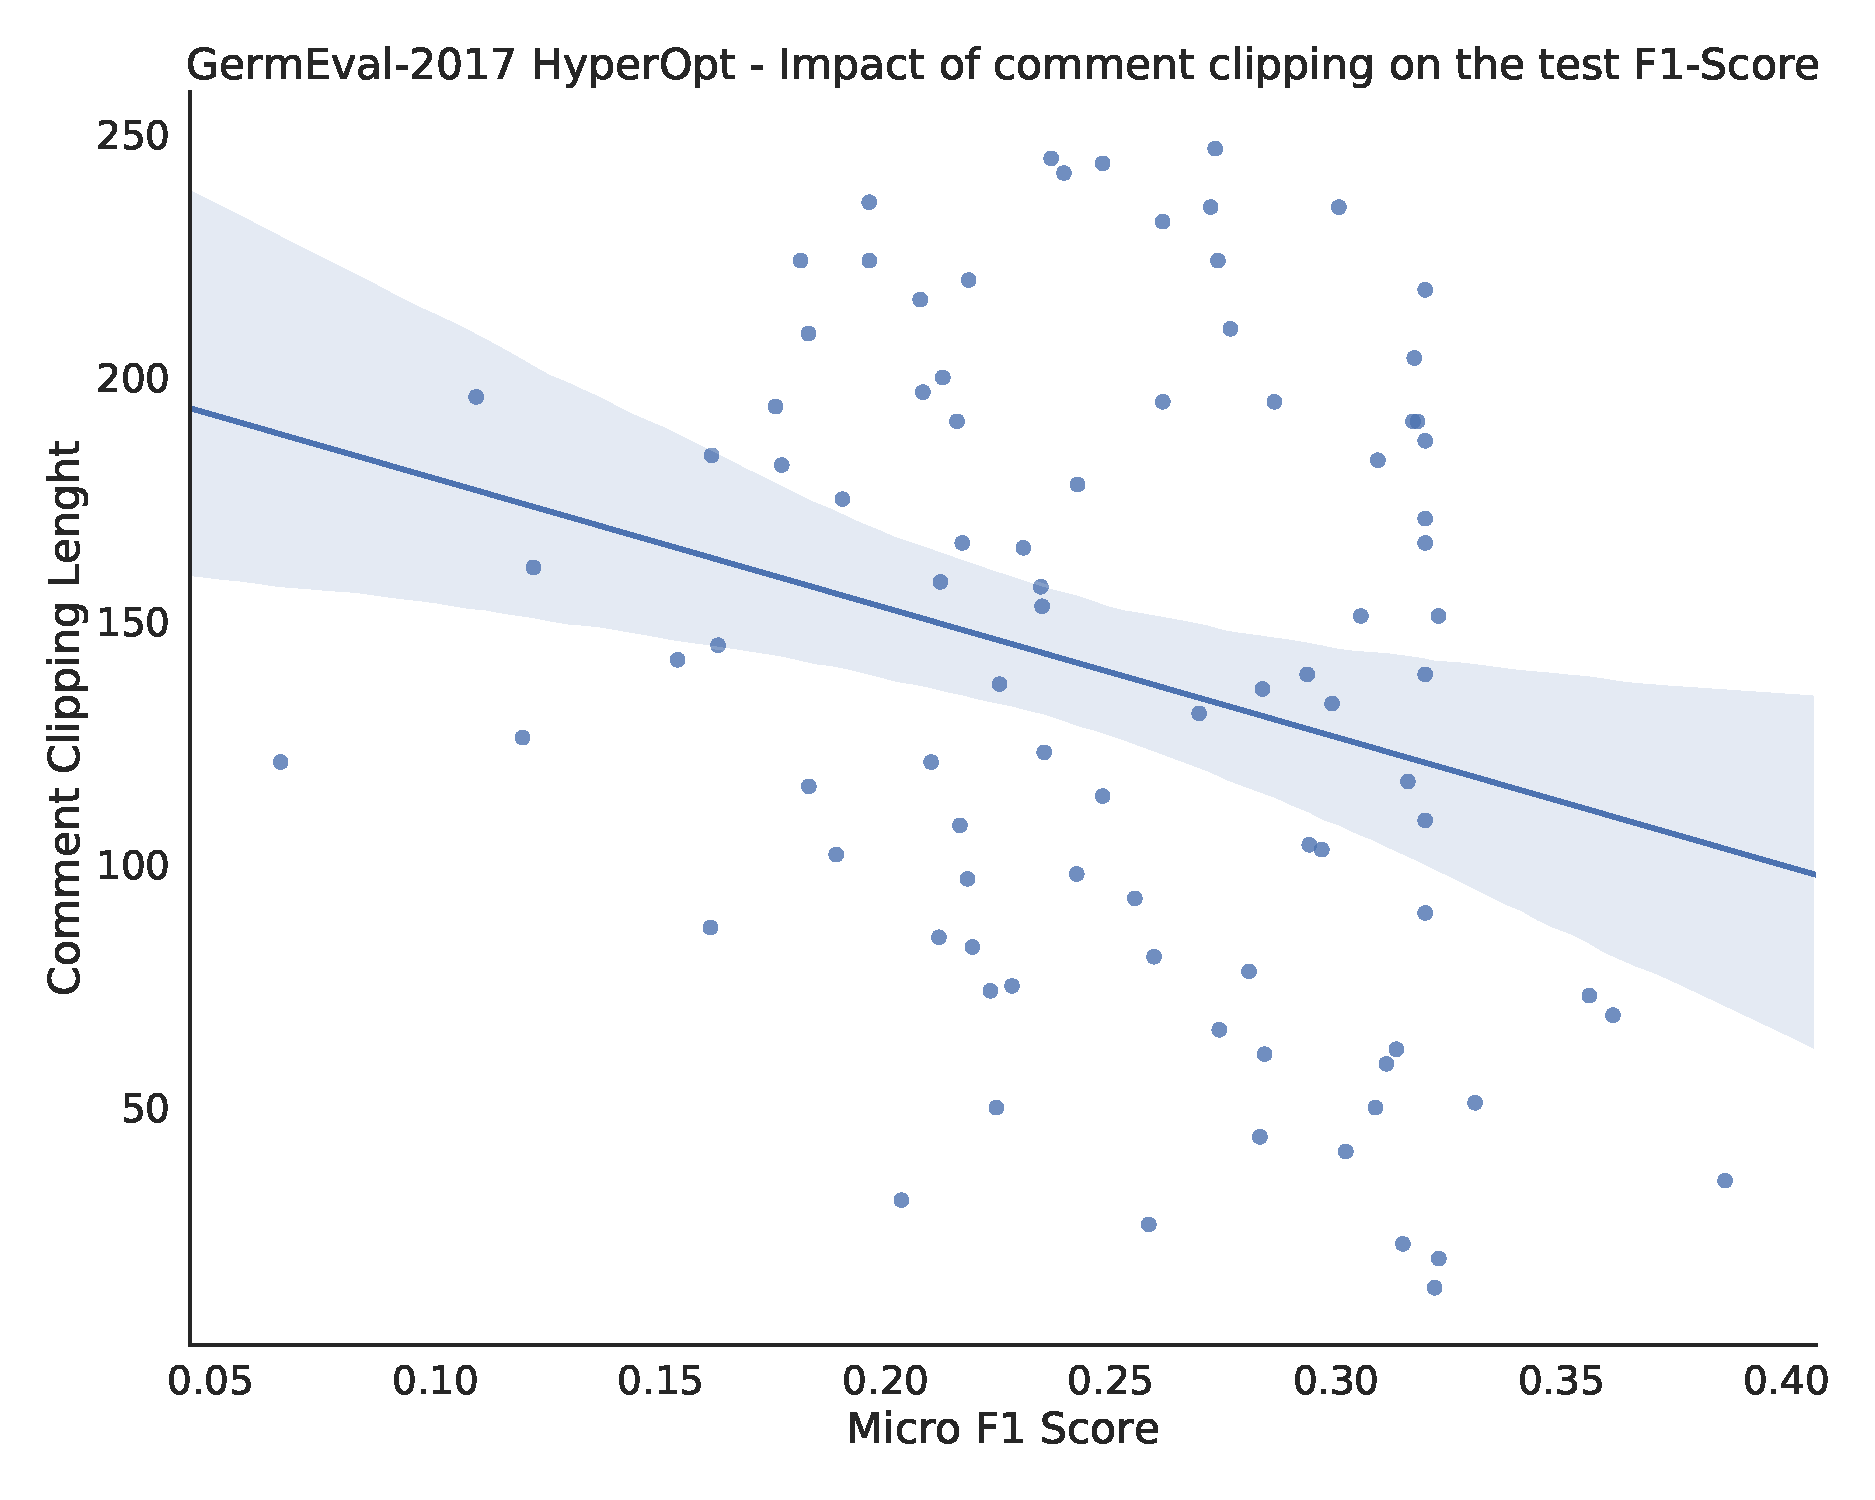
\includegraphics[width=\textwidth]{figures/06_results/06_hp_ge_lm_commentClipping_test}
	\caption{Comparison of preprocessing techniques - Impact of Comment Clipping on Test Micro F1-Score}
	\label{fig:06_PreprocessingCommentClipping}
\end{figure}

Comment clipping refers to the technique of cutting a sentence or comment after a specific number of tokens. In other words, comments which are too long are shortened and comments which are too short are padded.

Figure \ref{fig:06_PreprocessingCommentClipping} provides a visualization how comment clipping impacts the model performance on the GermEval-2017 dataset. The regression line shows that a shorter sequence length may improve performance of the overall model\footnote{Significant at a $p$-value of 0.05}.
\medskip

This observation seems to be reasonable since GermEval-2017 contains a mix of very short tweets {(140/280 character limit)} as well as long newspaper articles. Aligning them to an overall shorter length logical especially considering that most longer newspaper articles include a short summary in the beginning. Cutting those long documents helps the transformer to focus on important information instead of spreading out the attention.

\section{Results for Named Entity Recognition}

The following section contains the final results for the \acrfull{ner} task of the CoNLL-2003 dataset.

Since this task was an auxiliary training task to assess the performance of the transformer part, no hyperparameter tuning was performed.
\medskip

For this dataset the architecture is slightly different, because CoNLL-2003 has annotations for each word. Since the transformer makes predictions per word there is no need for separate aspect heads.

Therefore, this architecture follows the original transformer and consists of a single linear layer to project the 300-dimensional per-word prediction down to the amount of classes to predict. Finally, a log-softmax is used to provide the log probabilities for the class labels.
\medskip

For the final evaluations we use transformer model with two encoder blocks, each consisting of two attention heads. We employ a model dropout rate of 0.3 and a pointwise layer size of 300. Furthermore, we use FastText embeddings a batch size of 12 and a weight decay of $1e^-6$.

\begin{table}[]
	\centering
	\begin{tabular*}{\textwidth}{l@{\extracolsep{\fill}}cccc@{}}
	\toprule
	Variant          & \multicolumn{2}{c}{\textbf{Macro F1}}     & \multicolumn{2}{c}{\textbf{Micro F1}}       \\ 
	\midrule
					 & \textit{dev}      	& \textit{test} 		& \textit{dev}      		& \textit{test} 		\\
	\midrule
	Random Classifier          &  0.147   	& 0.187 	&  0.210  		&   0.214  \\
	CoNLL-2003 Baseline         &  -        	&  -    	& -        		&   0.596 		\\
	CoNLL-2003 Best Result & - & - & - & 0.888 \\
	Baevski et. al 2019 {(\gls{sota})} 		 & -        	& -    		& 0.969     	&   \textbf{0.935} 		\\
	Transformer {(our)}      & 0.822         	& 0.766	&  0.939        		&   0.918   			\\ \bottomrule
	\end{tabular*}
	\caption{Results of models on the shared CoNLL-2003 task for \gls{ner}. The random classifier acts as a minimal baseline as it will predict completely random classes for each sample. The CoNLL-2003 baseline \cite{Erik2003} was provided for the CoNLL-2003 NER competition. The best result at the competition achieved an F1-score of 0.8876 \cite{Florian2003}. At the time of writing {(April 2019)}, the best result on CoNLL-2003 NER is achieved by Baevski et. al. \cite{Baevski2019}}.
	\label{tab:06_resultsConLL}
	\end{table}

\bigskip
Table \ref{tab:06_resultsConLL} lists the result of our and other submissions for this tasks in order to assess the fitness of this model. The vanilla transformer model already achieves a very competitive performance. It outperforms every original submission for CoNLL-2013 by a wide margin and is only slightly behind current state of the art \cite{Baevski2019} even though it was not exclusively created for this purpose.
\medskip

\begin{figure}[ht]
	\centering
	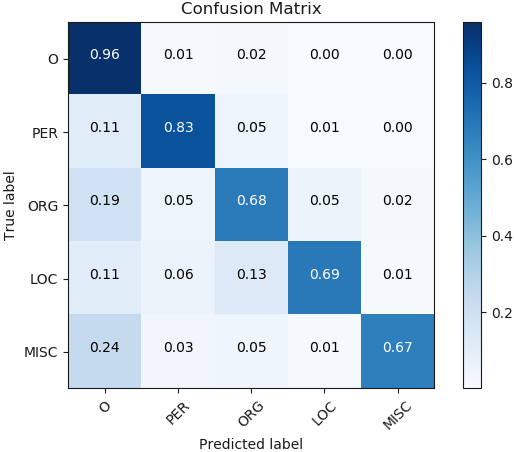
\includegraphics[width=0.49\textwidth]{figures/06_results/06_ner_final_test_c_matrix}
	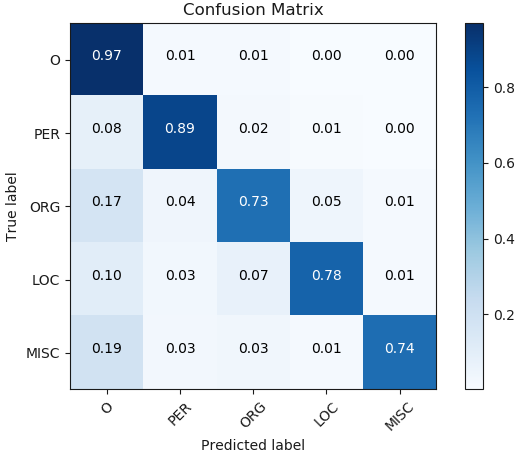
\includegraphics[width=0.49\textwidth]{figures/06_results/06_ner_final_valid_c_matrix}
	\caption{Normalized confusion matrices for the \gls{ner} task of the CoNLL-2003 dataset. The matrix on the left shows the performance of the model on the test set while the right confusion matrix visualizes the performance on the validation / development set.}
	\label{fig:06_NER_cmatrices}
\end{figure}

The normalized confusion matrices in figure \ref{fig:06_NER_cmatrices} show the performance of the transformer on the dataset for the individual classes. The class 'LOC' is the most frequent class in the dataset {(see table \ref{tab:05_conll2003DatasetStats})} aside from class 'O' which is the 'Other' class. Despite this fact, the class performed poorly considering the 'MISC' class which achieved a similar result only has half the training samples.



\section{Results for Aspect-Based Sentiment Analysis}
The following sections outline the results on \acrfull{absa}. The first section contains the results for the GermEval-2017 dataset. This dataset uses a special evaluation method. To be able to compare our results we also use the evaluation method that GermEval-2017 provides.

The method GermEval-2017 uses is described in section \ref{sec:05_GermEvalEvaluation}.
\medskip

Section \ref{sec:06_ResultsOrganic} reports results on the Organic-2019 dataset and section \ref{sec:06_ResultsAmazon} discusses the results on the Amazon Reviews dataset.

Finally, section \ref{sec:06_ResultsMultitask} and \ref{sec:06_ResultsTransfer} review the results of multitask learning and transfer learning.

\subsection{GermEval-2017}
\label{sec:06_ResultsGermEval}

\begin{table}[]
	\centering
	\begin{tabular*}{\textwidth}{l@{\extracolsep{\fill}}cccc@{}}
	\toprule
	Variant          & \multicolumn{2}{c}{\textbf{Macro F1}}     & \multicolumn{2}{c}{\textbf{Micro F1}}       \\ 
	\midrule
					 & \textit{synchronic test}      	& \textit{diachronic test} 		& \textit{synchronic test}      		& \textit{diachronic test} 		\\
	\midrule
	Random Classifier          		&  0.014   		& 0.014 	&  0.018  		&   0.018  \\
	Majority Baseline        	&  -        	&  -    	& 0.315        		&   0.384 		\\
	GermEval Baseline        	&  -        	&  -    	& 0.322        		&   0.389 		\\
	GermEval Best Result 		&  - 			&  - 		& 0.354 			& 0.401 \\
	Schmitt 2018 {(\gls{sota})} 		 & -        	& -    		& \textbf{0.423}     	&   \textbf{0.465} 		\\
	\midrule
	\gls{absat} + \gls{lmh}      & 0.131         	& -	&  0.390        		&   -   			\\ 
	\gls{absat} + \gls{cnnh}      & 0.822         	& -	&  0.939        		&   -   			\\ 

	
	\bottomrule
	\end{tabular*}
	\caption{Results of models on the shared CoNLL-2003 task for \gls{ner}. The random classifier acts as a minimal baseline as it will predict completely random classes for each sample. The CoNLL-2003 baseline \cite{Erik2003} was provided for the CoNLL-2003 NER competition. The best result at the competition achieved an F1-score of 0.8876 \cite{Florian2003}. At the time of writing {(April 2019)}, the best result on CoNLL-2003 NER is achieved by Baevski et. al. \cite{Baevski2019}}.
	\label{tab:06_resultsGermEval}
	\end{table}


\subsection{Organic-2019}
\label{sec:06_ResultsOrganic}

\subsection{Amazon Product Reviews}
\label{sec:06_ResultsAmazon}

Due to the large size of the dataset no hyperparameter tuning was performed. Parameters from previous optimizations on the smaller organic dataset were chosen for the evaluation. The final model uses the \gls{mlsa} architecture with fasttext embeddings. Comments are clipped to a fixed length of 100 and spell checking as well as stop word removal is enabled to reduce the vocabulary size. The model consists of one attention head with $d_k$ and $d_v$ of 300 and two encoder blocks. The inner \gls{pwfc}-layer acts as a bottleneck with a size of 128. Finally, a reduced batch size of 12 was chosen to be able to fit the model into \gls{gpu} memory which would not have been otherwise possible.
\medskip

The vocabulary size of the amazon dataset after all reductions consists of $389,371$ unique tokens. This creates an embedding layer which maps the vocabulary size of $389,371$ to a 300-dimensional vector. Unfortunately, a lot of those tokens are not part of the pretrained embedding so the parameters of the embedding layer can not be locked during training. Therefore, the embedding layer has a size of $116,811,300$ trainable parameters. As a result, the first embedding layer makes up over 99\% of the overall number of model parameters which is $117,710,780$.



\section{Impact of Multitask Learning}
\label{sec:06_ResultsMultitask}

Difference to Multitask learning

% additional gradient flow. Otherwise often only one aspect head. Now, at least two

\section{Impact of Transfer Learning}
\label{sec:06_ResultsTransfer}


